%\documentclass[dvipdfmx]{beamer}      % platex の場合
\documentclass[handout]{beamer}        % lualatex の場合
\usepackage{mySld}

\begin{document}
\title{基礎コンピュータ工学\\第2章 情報の表現\\
       (パート1:ビット)}
\date{}

\begin{frame}
  \titlepage
  \centerline{\url{https://github.com/tctsigemura/TecTextBook}}
  \vfill
  \centerline{本スライドの入手:
    \raisebox{-7mm}{
\includegraphics[scale=0.3]{../Img/QRs2_1.png}}}
\end{frame}

%==============================================================================
%\begin{frame}
%  \frametitle{}
%\end{frame}

\section{情報の表現}
%==============================================================================
\begin{frame}
  \frametitle{情報の表現}
  コンピュータの内部で情報が表現されるか.\\
  どのような回路で扱うことができるか.
  \vfill
  コンピュータは電気で動くので情報も電気で表現する必要がある.\\
\[ 情報の表現  =  \left(
\begin{tabular}{l}
  人 : 音声,文字,絵,... \\
  コンピュータ : 電圧,電流 \\
\end{tabular}
\right)\]
\end{frame}

%==============================================================================
\begin{frame}
  \frametitle{電気を用いた情報の表現(おおかみ情報)}
  電気の「ON/OFF」を用いて情報を表現する.
  \begin{center}
    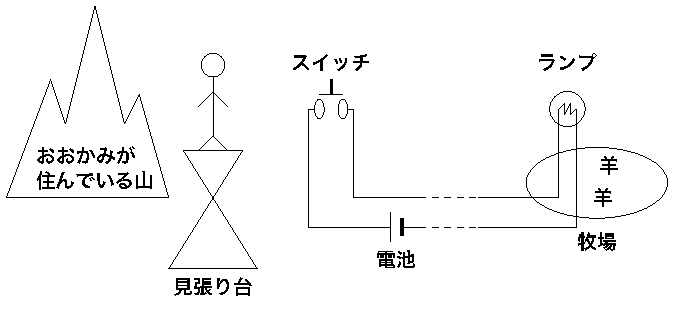
\includegraphics[scale=0.8]{../Tikz/ookami.pdf}
  \end{center}
  \begin{center}
    \begin{tabular}{l | l}\hline\hline
      ランプ  &  意 味 \\\hline
      OFF     & おおかみは来ていない \\
      ON      & おおかみが来た!!
    \end{tabular}
  \end{center}
\end{frame}

%==============================================================================
\begin{frame}
  \frametitle{おおかみ情報表示装置}
  牧場に次のような表示装置(カンバン)を設置する.
  \vfill
  \begin{center}
    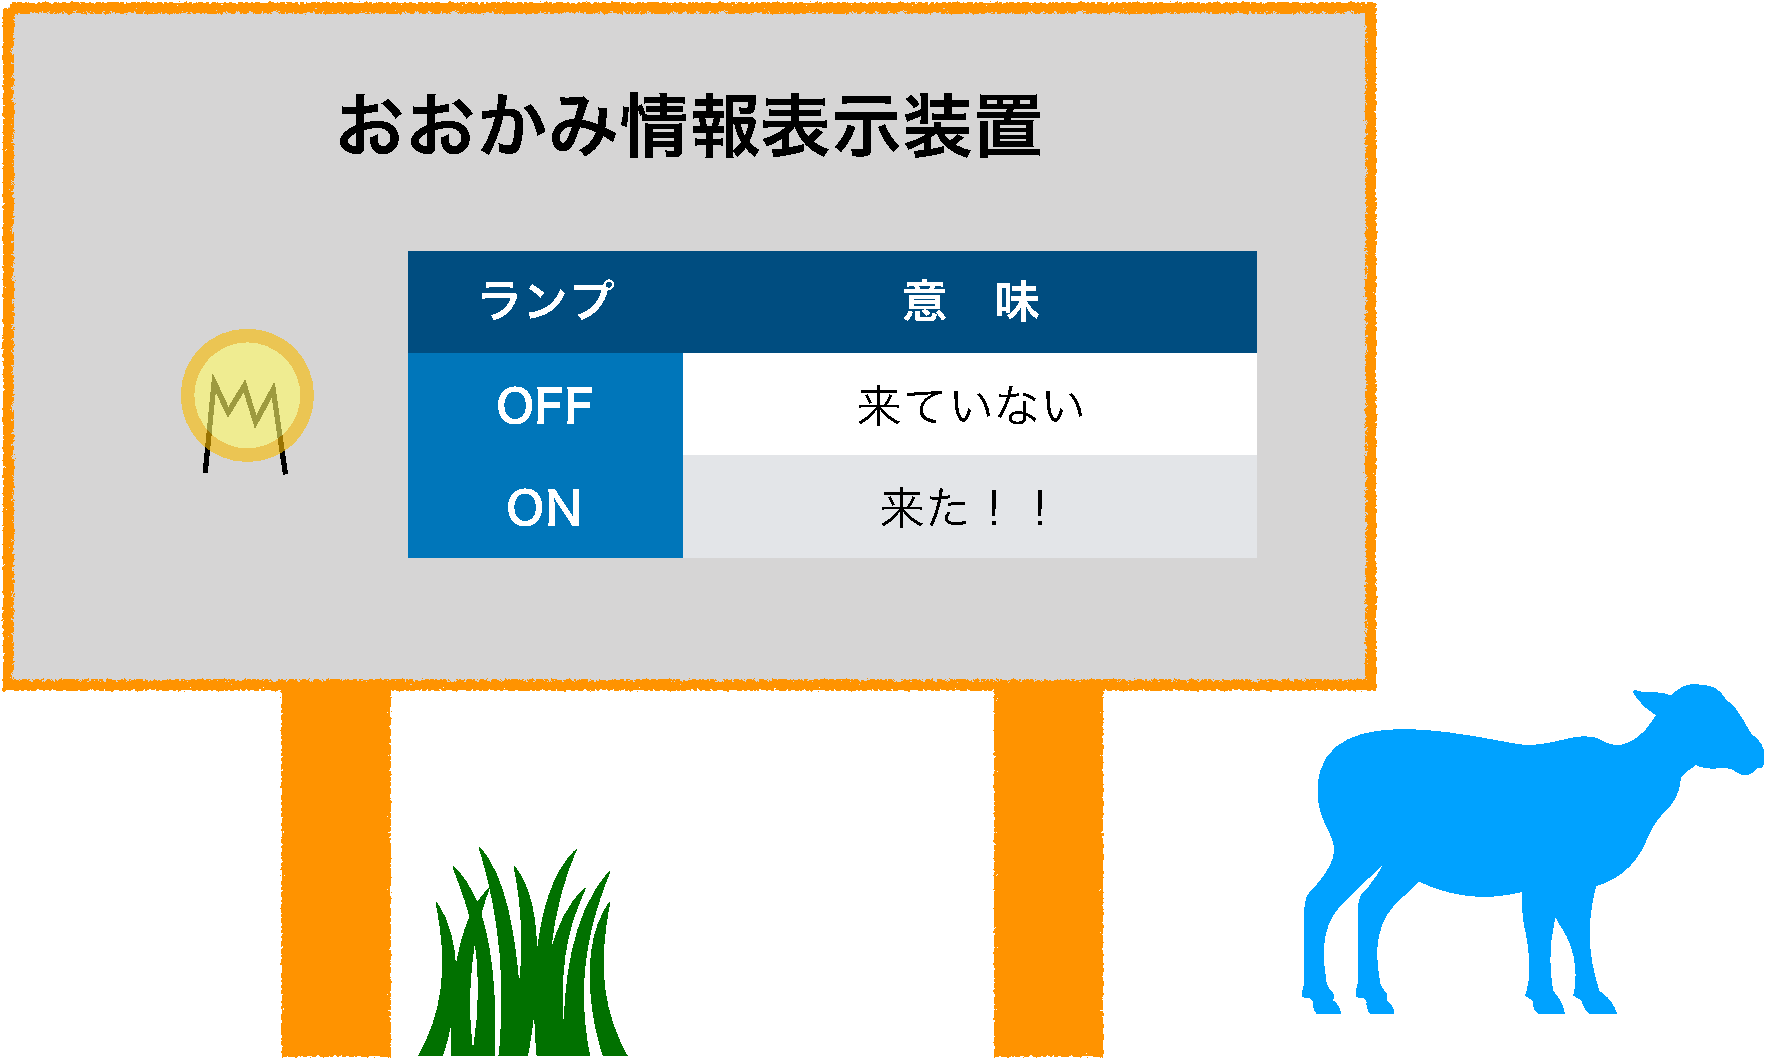
\includegraphics[scale=0.35]{Fig/display-crop.pdf}
    \vfill
  \end{center}
\end{frame}

%==============================================================================
\begin{frame}
  \frametitle{ビット}
  前例のような「二つのどちらか」を表す情報が「情報の最小単位」になる.
  情報の最小単位のことを「{\bf ビット(bit)}」と呼ぶ.

\begin{center}
\fbox{\parbox{0.9\columnwidth}{\small
{\bf on/offのどちらか → 情報の最小単位(ビット)}}}
\end{center}

ビットの値は「ON/OFF」ではなく,「1/0」で書く.
\begin{center}
{\small\[\left(\begin{tabular}{l c l}
ON  & : & 1 \\
OFF & : & 0
\end{tabular}\right)\]}
\end{center}

「おおかみが来た情報」をビットで表現する.
  \begin{center}
    \begin{tabular}{l | l}\hline\hline
      ビット値  &  意 味 \\\hline
      0(off)  & おおかみは来ていない \\
      1(on)   & おおかみが来た!!
    \end{tabular}
  \end{center}

\end{frame}

%==============================================================================
\begin{frame}
  \frametitle{より複雑な情報の表現(拡張おおかみ情報)}
  複雑な情報は複数のランプ(ビット)の組み合わせで表現する.
  \begin{center}
    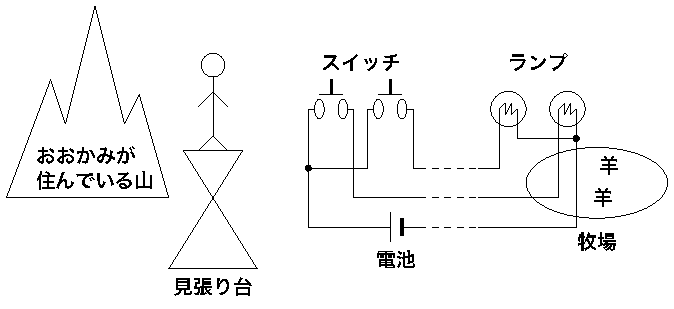
\includegraphics[scale=0.8]{../Tikz/ookami2.pdf}
    {\small\begin{tabular}{c|l} \hline\hline
      ビット値 & \multicolumn{1}{c}{意 味}  \\
      \hline
      00 & おおかみはきていない(平気)      \\
      01 & おおかみが1頭来た(戦う)         \\
      10 & おおかみが2頭来た(?)           \\
      11 & おおかみがたくさん来た(逃げる)  \\
    \end{tabular}}
  \end{center}
\end{frame}

%==============================================================================
\begin{frame}
  \frametitle{拡張おおかみ情報表示装置}
  牧場に次のような表示装置(カンバン)を設置すればよい!!
  \vfill
  \begin{center}
    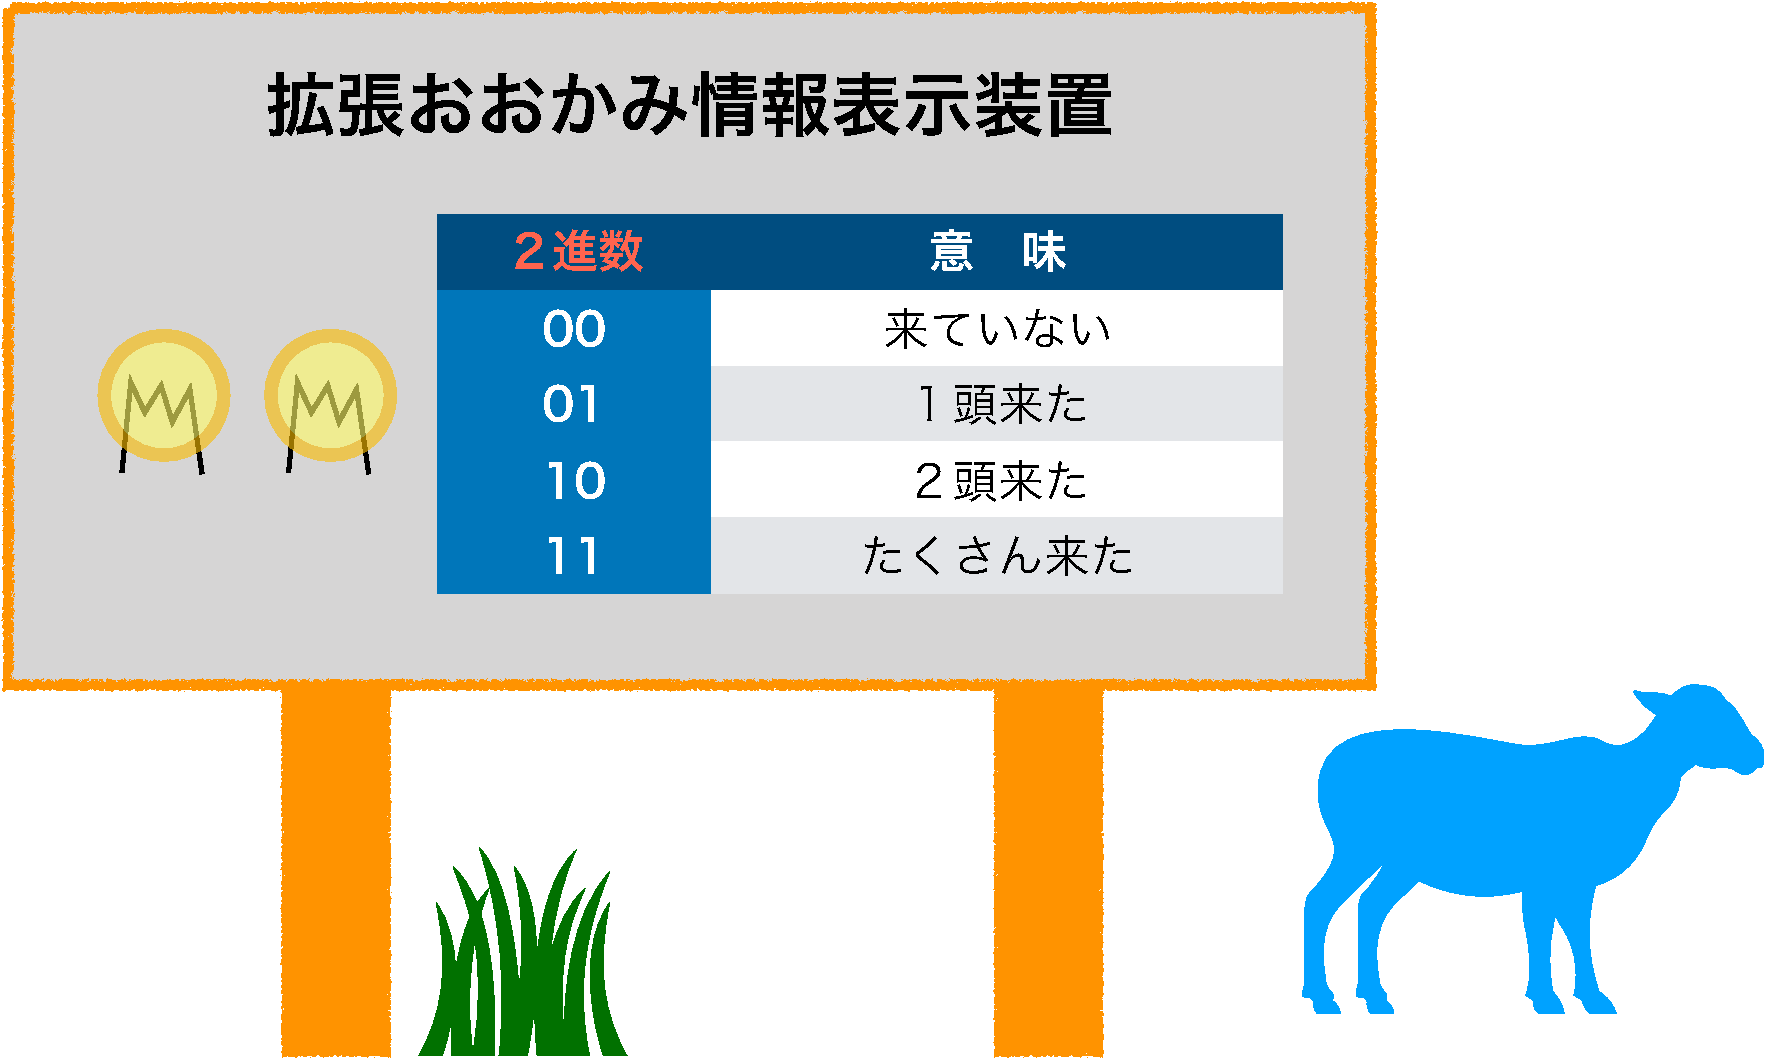
\includegraphics[scale=0.35]{Fig/display2-crop.pdf}
    \vfill
  \end{center}
\end{frame}

%==============================================================================
\begin{frame}
  \frametitle{ビットの組合せと表現できる情報}
  拡張おおかみ情報は2ビットで4種類の情報を表現した.
  一般には$n$ビットで$2^n$種類の情報を表現できる.
  \begin{center}
    {\small\begin{tabular}{c|l|l} \hline\hline
      ビット数 & \multicolumn{1}{c|}{ビットの組合せ} & 組合せ数\\
      \hline
      1 & 0 1   & $2^1$ ($=2$) \\
      2 & 00 01 10 11 & $2^2$ ($=4$) \\
      3 & 000 001 010 011 &   \\
      & 100 101 110 111 & $2^3$ ($=8$) \\
      ...& ... &\\
      n &  & $2^n$ \\
    \end{tabular}}
  \end{center}

  「拡張おおかみ情報」のように,
  ビットの組合せに意味を持たせることで様々な情報を表現できる.
  \begin{center}
    {\bf ビットの組合せの意味を表にして定義する.}
  \end{center}
\end{frame}

%==============================================================================
\begin{frame}
  \frametitle{ビット,ニブル,バイト}
  「ビット」は情報の最小単位 \\
  「ビット」は小さすぎるので「4ビット」,「8ビット」まとめたものもある.

  \begin{center}
    \begin{tabular}{c|l|l} \hline\hline
      名前 & ビット数 & 組合せの数\\
      \hline
      ビット(bit)    & 1   & $2^1 = 2$ \\
      ニブル(nibble) & 4   & $2^4 = 16$ \\
      バイト(byte) & 8   & $2^8 = 256$ \\
    \end{tabular}
  \end{center}

  スマホの容量:32GB,64GB,128GB(「B」は{\bf バイト}の意味) \\
  USBメモリの容量:32GB,64GB,128GB(「B」は{\bf バイト}の意味) \\
  通信速度制限:7GB を超えると制限される(「B」は{\bf バイト}の意味) \\
  通信速度:通常は 100Mbps(「b」は{\bf ビット}の意味) \\
  通信速度:制限されると 128kbps(「b」は{\bf ビット}の意味) \\

  参考: bps : 【bits per second / ビット毎秒】
\end{frame}

%==============================================================================
\begin{frame}
  \frametitle{数値の表現}
  これまで,ビットの組合せの意味決める.(表などにする) \\
  ビットの組合せの意味を{\bf ルールで決める}場合もある.\\
  コンピュータの内部では数値は{\bf 2進数}で表現する.

  {\bf 10進数} \\
  \begin{itemize}
    \item 0〜9の10種類の数{\bf 字}だけを使用する数値の表現方法.
    \item 一桁毎に10倍の重みを持つ
  \end{itemize}

  {\bf 2進数} \\
  \begin{itemize}
    \item 0,1の2種類の数{\bf 字}だけを使用する数値の表現方法.
    \item 一桁毎に2倍の重みを持つ
    \item 0,1の2種類の数字を{\bf ビットの0,1と対応付け}しやすい.
    \item $n$ビット(桁)の2進数で$0$〜$2^n-1$までの値を表現できる.
  \end{itemize}

\end{frame}

%==============================================================================
\begin{frame}
  \frametitle{4ビットの2進数}
  \begin{center}
    {\small\begin{tabular}{c|c|c|c|r}
      \hline\hline
      $b_3$ & $b_2$ & $b_1$ & $b_0$ & 意味\\
      \hline
      0 &  0 &  0 &  0 &  0 \\
      0 &  0 &  0 &  1 &  1 \\
      0 &  0 &  1 &  0 &  2 \\
      0 &  0 &  1 &  1 &  3 \\
      0 &  1 &  0 &  0 &  4 \\
      0 &  1 &  0 &  1 &  5 \\
      0 &  1 &  1 &  0 &  6 \\
      0 &  1 &  1 &  1 &  7 \\
      1 &  0 &  0 &  0 &  8 \\
      1 &  0 &  0 &  1 &  9 \\
      1 &  0 &  1 &  0 & 10 \\
      1 &  0 &  1 &  1 & 11 \\
      1 &  1 &  0 &  0 & 12 \\
      1 &  1 &  0 &  1 & 13 \\
      1 &  1 &  1 &  0 & 14 \\
      1 &  1 &  1 &  1 & 15 \\
    \end{tabular}}
  \end{center}
\end{frame}

%==============================================================================
\begin{frame}
  \frametitle{宿題}

\emph{宿題}
\begin{enumerate}
\item[1)] 言葉の確認(ビット、ニブル、バイト)
\vfill
\item[2)] n ビットの組合せの数 \\
  3ビットで表現できる情報の種類は何種類か? \\
  32種類の情報表現するためには何ビット必要か?
\vfill
\item[3)] $0_{10}$($0000_2$) 〜 $15_{10}$($1111_2$)の範囲を \\
  2進数で数を数える練習をしなさい.\\
  (小学校の1年生が10まで数える練習をするように)
\vfill
\end{enumerate}
\end{frame}

\end{document}
